\documentclass{article}
\setcounter{secnumdepth}{0} % removes numeration of (sub)sections
\usepackage{hyperref} %snel klik in pdf linkjes
\usepackage{graphicx} 
\usepackage[dutch,english]{babel}
\usepackage{graphicx}
% ref packages
\usepackage{nameref}
% folowing  must be in this order
\usepackage{varioref}
\usepackage{hyperref}
\usepackage{cleveref}

\usepackage[table,xcdraw]{xcolor}
\usepackage[normalem]{ulem}
% \usepackage{flafter} prevents figures ever floating backwards up the current page
%\useunder{\uline}{\ul}{}
\graphicspath{ {./images/} }
\begin{document}
\sffamily



\begin{titlepage}
  \centering
    \vfill
    {\bfseries\Huge
      EindVerslag Tinlab Advanced Algorithms \\
        \vskip2cm
      }
      {\bfseries\Large
        Studenten:\\
      }
      {
        \bfseries\normalsize
        Jordi Luijk 0889529 \newline
        Emre Tukuc 08772624 \newline\\
        \vskip1cm
        \today\\
    }    
    \vfill
    
\includegraphics[width=4cm]{logohr.png} % also works with logo.pdf
    \vfill
    \vfill
\end{titlepage}
\newpage
\tableofcontents

\newpage
%\section{Voorwoord}
%\newpage
\section{Versiebeheer}

\begin{table}[htp]
\begin{tabular}{llll}
\rowcolor[HTML]{FFD700} 
{\ul \textbf{Versie nr}} & {\ul \textbf{Veranderingen}} & {\ul \textbf{Datum}} & {\ul \textbf{Auteur}} \\
0.1 & Initieel Concept & 17-3-'19 & J.Luijk \\     
a & b & c & d \\     
a & b & c & d   
\end{tabular}
\end{table}
\newpage

\section{Verklarende woordenlijst}
\textbf{Schutkolk of sluiskolk} \newline
De ruimte tussen twee sluisdeuren, wordt gebruikt om boten te leiden van de ene naar de andere \cite{definitionschutkolk}.
\newpage
\section{Introductie}
\subsection{Probleemstelling}
Er moet een model worden ontwikkeld voor een sluis. Dit model moet abstract genoeg zijn om te kunnen worden ingezet in meerdere situaties. Technische besluiten zoals het aantal sluizen, waterniveaus en de regeling daarvan worden door onderzoek bepaald.

\subsection{Meerwaarde van het onderzoek}
Het resultaat van het onderzoek zal de stakeholder betere grip geven op het gebied van ict en systemen en hun mogelijkheden op deze gebieden vergroten. 

\subsection{Stakeholders}
Ministerie van Infrastructuur en Waterstaat is geïnteresseerd in een modellen die ze mogelijk kunnen integreren in het huidige infrastructuur.

\section{Theoretisch Kader}
In dit hoofdstuk wordt informatie verzameld en concepten behandel voor het realiseren van het sluis model.

\subsection{De Kripke structuur}

Kripke structuren zijn een manier om het gedrag van een systeem te modelleren. Belangrijke termen voor het bespreken van Kripke structuren zijn states en transities. \newline

Een state beschrijft de toestand waarin een systeem zich bevindt. In het geval dat de state niet duidelijk is voor de gebruiker dan wordt dat mode confusion genoemd. Transities zijn de overgangen van één state naar de anderen. 

\begin{figure}[!h]
	\centering
	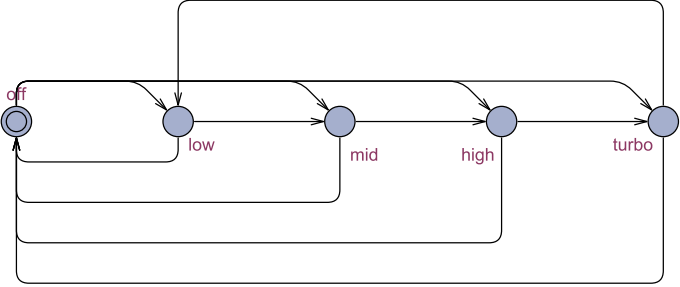
\includegraphics[width=\textwidth]{kripke_structure_example1}
    \caption{Voorbeeld Kripke structuur}
	%\label{fig:figure2}
\end{figure}

\subsection{Soorten modellen} \label{SoortenModellen}

\textbf{World vs. machine:} 
\\
Er kan onderscheid worden gemaakt tussen de fenomenen die zich bevinden in de wereld buiten het systeem en de fenomenen die alleen in het systeem zelf bestaan. Deze verschillen verschilt voor elke machine, het hangt volledig af van welke inputs en outputs de machine heeft. Een simpele voorbeeld van wereldse fenomeen is het temperatuur en een fenomeen die alleen in het machine bestaat is het programma waar het machine op functioneert. \\\\
\textbf{4 variabelen methode:}
\\
Modellen voor computer systemen gebruiken vaak antropomorfisme analogie en intuïtieve conclusies wat tot lager precisie kan leiden. Het vier variabelen model helpt om software vereisten met groter precisie vast te stellen, door deze te modelleren op een manier zoals vaak door ingenieurs wordt toegepast. \cite{parnas1995functional} 
\\\\
Zoals de naam suggereert bestaat het vier variabelen model uit vier onderdelen. Input, output, gecontroleerde variabelen en gemonitorde variabelen. Als eerste de gemonteerde variabelen die buiten het systeem bestaan en worden opgenomen door sensoren, waarna deze input is voor de software. Deze input draagt bij aan de output of acties die het systeem in de buitenwereld creëert, de resultaten hiervan heten de gecontroleerde variabelen. Zie ook Figuur ~\ref{fig:four_Variables} hieronder.


\begin{figure}[!h]
	\centering
	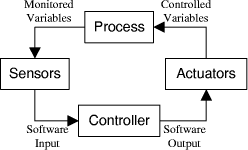
\includegraphics[width=\textwidth]{four_Variables}
    \caption{Vier variabelen model \cite{thompson2000requirements}}
	\label{fig:four_Variables}
\end{figure}

\subsection{Tijd}
In Uppaal wordt tijd globaal op hetzelfde tempo bijgehouden. Tijd wordt in klokken bijgehouden en kan op elk moment worden uitgelezen of gereset. Tijd in uppaal heeft geen vaste eenheid en er kunnen verschillende eenheden toegewezen worden zolang het wek consistent word uitgevoerd. \cite{uppaalsmalltutorial}
\subsection{Guards en invarianten}
Guards zijn condities die op transities worden geplaatst, aan deze condities moet worden voldaan voordat deze transitie mogelijk is. Een van de vele condities die je kan definiëren is het verstrijken van een bepaalde eenheid tijd voordat het die transitie mag aan ingaan. \cite{uppaalsmalltutorial}

\subsection{Deadlock} \label{deadlock}

Een deadlock is een situatie waarin er nooit meer verdere state transities mogelijke zijn. Dit zorgt ervoor dat het systeem volledig stil staat en niks meer kan doen. Deadlocks kunnen ontstaan door door bepaalde condities te definiëren die het systeem niet kan waarmaken \cite{uppaalintro}.

\subsection{Zeno gedrag} \label{zenobehavior}
Wanneer een model een oneindig aantal transities kan maken in een bepaalde tijd dat wordt er gesproken van zeno gedrag. \cite{uppaaltutorialmodelingpatterns} \cite{leine2011zeno}.

\subsection{Waterniveau}

In een document waarin informatie over de vaarwegen in Nederland zijn verzameld, is een standaard aangehouden van 2,45 meter en 1,10 meter voor respectievelijk de doorvaarthoogte en diepte \cite{vaarwegennederland2017}. 

\section{Onderzoeksresultaten}

\subsection{Vereisten}

De sluis is een schutsluis wat betekent dat deze in staat is om boten van de een naar de andere kant, door de schutkolk heen, te leiden. De sluis moet volautomatisch kunnen opereren. Dit houd in dat de sluis zelf de benodigde waterniveau bepalen en aanpassen. De sluis deuren moeten vol automatisch open en dicht gaan zonder obstakels er tussen.


\subsection{Requirements / Functionaliteiten-lijst}\label{sec:FuncList}
\textbf{ID: F1} \newline
\textbf{Functionaliteit: Openen en sluiten van de sluisdeur(en)} \newline
De sluisdeur(en) moeten in staat zijn om open en dicht te gaan in een realistische tijd. \newline

\textbf{ID: F2} \newline
\textbf{Functionaliteit: Waterniveau detecteren} \newline
Het water niveau aan beide kanten van de sluis en binnen de sluiskolk moet kunnen worden gedetecteerd. \newline

\textbf{ID: F3} \newline
\textbf{Functionaliteit: Waterniveau reguleren} \newline
Het water niveau in de sluiskolk moet door middel van pompen kunnen worden verhoogd of verlaagt. \newline

\textbf{ID: F5} \newline
\textbf{Functionaliteit: Boten moeten kunnen signaleren dat zei willen oversteken} \newline
Door middel van een signaal weet de sluis welke sluisdeuren deze moet open. \newline

\textbf{ID: F6} \newline
\textbf{Functionaliteit: Sluisdeuren kunnen niet sluiten als er een obstakel in de weg zit} \newline
Obstakel kan een boot zijn. Voor de veiligheid van deze boten moeten de sluisdeuren niet kunnen sluiten totdat obstakels zijn verwijderd.  \newline

\textbf{ID: F7} \newline
\textbf{Functionaliteit: Beide sluisdeuren kunnen niet tegelijk open zijn.} \newline
Een situatie waarin dit gebeurd zou bij goed functioneren niet optreden. Desondanks zal deze wel worden gemoduleerd. \newline


\section{Realisatie/Proof of Concept}

\subsection{Technische besluiten}
\textbf{Aantal sluizen}\newline
Er is gekozen om twee sluisdeuren te modelleren omdat dit complex genoeg is om een model te vereisen en omdat deze genoeg mogelijkheden openhoudt voor enige uitbreidingen. Het model zal zoals in de functionaliteiten-lijst aangegeven op pagina \pageref{sec:FuncList} waterniveau bijhouden en boten door de sluiskolk kunnen leiden.\\\\
Zie Figuur \ref{fig:sluiceWaterLv} voor een afbeelding hiervan. 
\begin{figure}[!h]
	\centering
	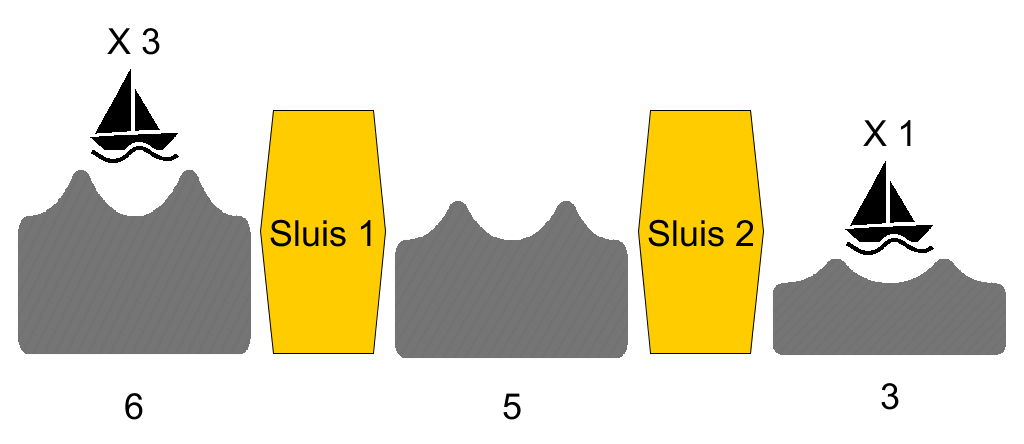
\includegraphics[width=\textwidth]{images/sluis_model.png}
    \caption{Model sluis dat twee sluisdeuren bevat en waterniveau bevat.}
	\label{fig:sluiceWaterLv}
\end{figure}

\noindent\textbf{Waterniveau aanpassen}\newline
Het waterniveau word aangepast door middel van een water pomp. Deze water pomp moet water in of uit het sluiskolk pompen wanneer er daar een signaal voor gegeven word.\newline

\noindent\textbf{Detectie boten tussen sluisdeuren}\newline
Detectie of boten nog tussen de sluisdeuren zitten word gedaan door twee setjes van tien tal infrarood sensoren en receivers die geplaatst worden aan de binnenkant van iedere sluisdeur. Met deze methode kan het sluis detecteren of de infrarood sensoren worden geblokkeerd door een object. Zodra de receivers geen signaal meer krijgen betekend het dat er een boot tussen de deuren zit.\newline

\noindent\textbf{Aanmeld systeem}\newline
Voor het aanmeld systeem is er besloten om een sms systeem op te zetten. Deze systeem krijgt via sms aanmeldingen binnen en die worden vervolgens in het wachtrij gezet in het systeem. \newline

\noindent\textbf{Waterniveau detecteren}\newline
\newline Om het waterniveau te detecteren is er gekozen om vier tal sensoren te gebruiken. Twee hiervan worden geplaatst in het sluiskolk en twee ervan buiten de sluis. De sensoren moeten in paren gezien worden een voor de eerste sluis deur en een voor de tweede deur. Elke paar sensoren moeten op de zelfde hoogte geplaatst worden dat bepaald word door het waterniveau aan de respectieve kant. Deze sensoren meten hoe hoog het water staat, deze sensoren meten niet de totale waterniveau, er word alleen gemeten hoe hoog het staat relatief aan het sensor, in figuur \ref{fig:sluiceSensoren} kunt u duidelijker zien wat hiermee word bedoeld sensoren worden afgekort met een S. De sensoren hebben 5 meetpunten even verdeeld over de hele lengte van de sensor.
\begin{figure}[!h]
	\centering
	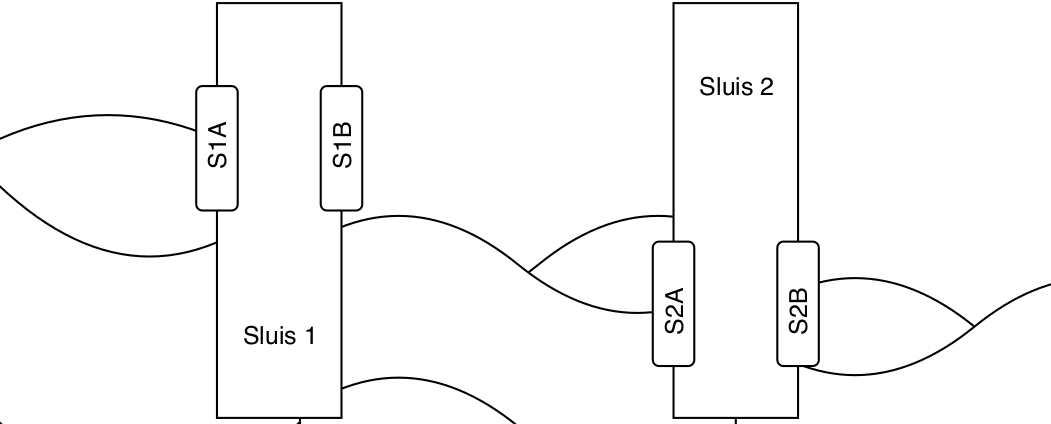
\includegraphics[width=\textwidth]{images/sluis_sensoren.png}
    \caption{Model sluis met positie sensoren.}
	\label{fig:sluiceSensoren}
\end{figure} \newpage



\subsection{Ontwerpen}
//screen capture Uppaal model \newline

1) Waterniveau in sluiskolk gelijkmaken aan links \newline
2) Deuren links openen \newline
3) boten de sluiskolk in \newline
4a) opt: check of deuren dicht kunnen, geen obstructie \newline
4b) deuren links dicht \newline
5) waterniveau verlagen naar die van de rechter kant \newline
6) Deuren links openen \newline
7a) boten uit de sluiskolk \newline
7b) nieuwe boten van de rechter kant binnenlaten \newline
8a) opt: check of deuren dicht kunnen, geen obstructie \newline
8b) deuren rechts dicht \newline

Onderdelen templates: \newline
Sluisen \newline
Sensoren (water niveau) \newline
Actuatoren (licht, opt: geluid) \newline
Pompen


\subsection{Testen}

De kwaliteit van het gerelaiseerde model wordt gewaarborgd aan de hand van de functionaliteiten, beschreven onder '~\nameref{sec:FuncList}' op pagina ~\pageref{sec:FuncList}. Dit betekent dat er getest wordt op functionaliteit, daarnaast zullen ongewilde situaties zoals deadlocks (zie pagina \pageref{deadlock}) en zeno gedrag (zie pagina \pageref{zenobehavior}) onmogelijk gemaakt worden.

\subsubsection{Resultaten}

Er is op X functionaliteiten getest. De lijst van functionaliteiten en hun beschrijving is te vinden onder \nameref{sec:FuncList} voor gekozen oplossing op pagina \pageref{sec:FuncList}. De functionaliteiten zijn genummerd van F1 tot en met FX.

De functionaliteiten zijn genoteerd als werkend in de aanwezigheid van de ingenieur.

\begin{table}[htp]
\begin{tabular}{llllll}
\rowcolor[HTML]{FFD700} 
{\ul \textbf{Id nr.}} & {\ul \textbf{Actie}} & {\ul \textbf{Input}} & {\ul \textbf{Verwachte output}} & {\ul \textbf{Output}} & {\ul \textbf{Pass/No pass}} \\
F1 & Initieel Concept & input & v. output & output & No pass \\     
F1 & Initieel Concept & input & v. output & output & No pass \\ 
F1 & Initieel Concept & input & v. output & output & No pass
\end{tabular}
\end{table}

\section{Bijlagen}
\newpage
\bibliography{references}
\bibliographystyle{plain}


\end{document}


